\documentclass[12pt]{article}

\usepackage{listings}
\usepackage[swedish]{babel}
\usepackage[T1]{fontenc}
\usepackage[utf8]{inputenc}
\usepackage{graphicx}
\usepackage{mathtools}
\usepackage{times}
\usepackage{url}
\usepackage{color}

\title{Rapport för laboration i digital ljudsyntes}

\author{
    \textbf {Marc Coquand} (författare) \\
    maco0044 \\
    mcoquand@gmail.com\\
    \and
    Oskar Olausson \\
    osol0010 \\
    oskar.erik.olausson@gmail.com\\
}
\date{\today}
\definecolor{mygreen}{rgb}{0,0.6,0}
\definecolor{mygray}{rgb}{0.5,0.5,0.5}
\definecolor{mymauve}{rgb}{0.58,0,0.82}

\lstset{ %
  backgroundcolor=\color{white},   % choose the background color; you must add \usepackage{color} or \usepackage{xcolor}
  basicstyle=\footnotesize,        % the size of the fonts that are used for the code
  breakatwhitespace=false,         % sets if automatic breaks should only happen at whitespace
  breaklines=true,                 % sets automatic line breaking
  captionpos=b,                    % sets the caption-position to bottom
  commentstyle=\color{mygreen},    % comment style
  deletekeywords={...},            % if you want to delete keywords from the given language
  escapeinside={\%*}{*)},          % if you want to add LaTeX within your code
  extendedchars=true,              % lets you use non-ASCII characters; for 8-bits encodings only, does not work with UTF-8
  frame=single,	                   % adds a frame around the code
  keepspaces=true,                 % keeps spaces in text, useful for keeping indentation of code (possibly needs columns=flexible)
  keywordstyle=\color{blue},       % keyword style
  language=Octave,                 % the language of the code
  otherkeywords={*,...},           % if you want to add more keywords to the set
  numbers=left,                    % where to put the line-numbers; possible values are (none, left, right)
  numbersep=5pt,                   % how far the line-numbers are from the code
  numberstyle=\tiny\color{mygray}, % the style that is used for the line-numbers
  rulecolor=\color{black},         % if not set, the frame-color may be changed on line-breaks within not-black text (e.g. comments (green here))
  showspaces=false,                % show spaces everywhere adding particular underscores; it overrides 'showstringspaces'
  showstringspaces=false,          % underline spaces within strings only
  showtabs=false,                  % show tabs within strings adding particular underscores
  stepnumber=2,                    % the step between two line-numbers. If it's 1, each line will be numbered
  stringstyle=\color{mymauve},     % string literal style
  tabsize=2,	                   % sets default tabsize to 2 spaces
  title=\lstname                   % show the filename of files included with \lstinputlisting; also try caption instead of title
}

\begin{document}
\lstset{language=Matlab}
\maketitle
\tableofcontents

\newpage

\section{Inledning och problembeskrivning}

Målsättningen med denna laborationen är att få fördjupande kunskaper i digital
signalhantering genom att lära sig de grundläggande principerna för digital
ljudsyntes av strängliknande instrument. Detta gjordes genom att läsa in en bild
i Matlab som innehåller information om vilka toner som ska spelas upp och
tonernas spacing. 

Vi skapade därför ett tonbibliotek och satte samman tonerna till en låt.
Därefter sparade vi låten till HD.


\section{Genomförande}

Uppgiften utfördes genom att man utvecklade ett program i Matlab som läser in en
bild, konverterar bilden till information om vilka toner som ska spelas upp och
tonernas spacing. Låten som valdes var en gotländsk polska som heter skaffare,
bilden som beskriver låten syns i figur~\ref{fig:skaffare}

\begin{figure}[!htb]
    \centering
    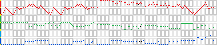
\includegraphics[scale=1.5]{../SKAFFARE.png}
    \caption{Bilden som innehåller informationen om låtens toner och spacing}
    \label{fig:skaffare}
\end{figure}

Varje pixel representerar en ton, färger som har RGB-värden högre än
$(200,200,200)$ ignoreras och en helsvart pixel läses in som en halvton högre än
pixels normala värde. 

Programmet accepterar upp till 3 spår. Varje spår är 15 höjd och börjar på
varandra. Pixeln högst upp i varje spår representerar högsta tonen och pixeln
lägst ner i varje spår representerar lägsta tonen.

Efter att programmet konverterat bilden så läser den in varje spår och därefter
konverterar det till rätt skala (bilden är i kromatisk skala annars). Där skapar
den också tonerna med funktionen \texttt{newTone.m} vars källkod finns i bilagor.

Sist lägger den ihop alla kanaler till ett spår till en låt och normaliserar.
Därefter sparar den låten.

Beskrivning om teorin bakom tonljuden hittas i bilagor.

\section{Resultat}

Den färdiga låten hittas på \url{https://github.com/oskarOlausson/Ljudprojekt/}
i \texttt{MATLAB/skaffare.mp3}. 

\begin{figure}[!htb]
    \centering
    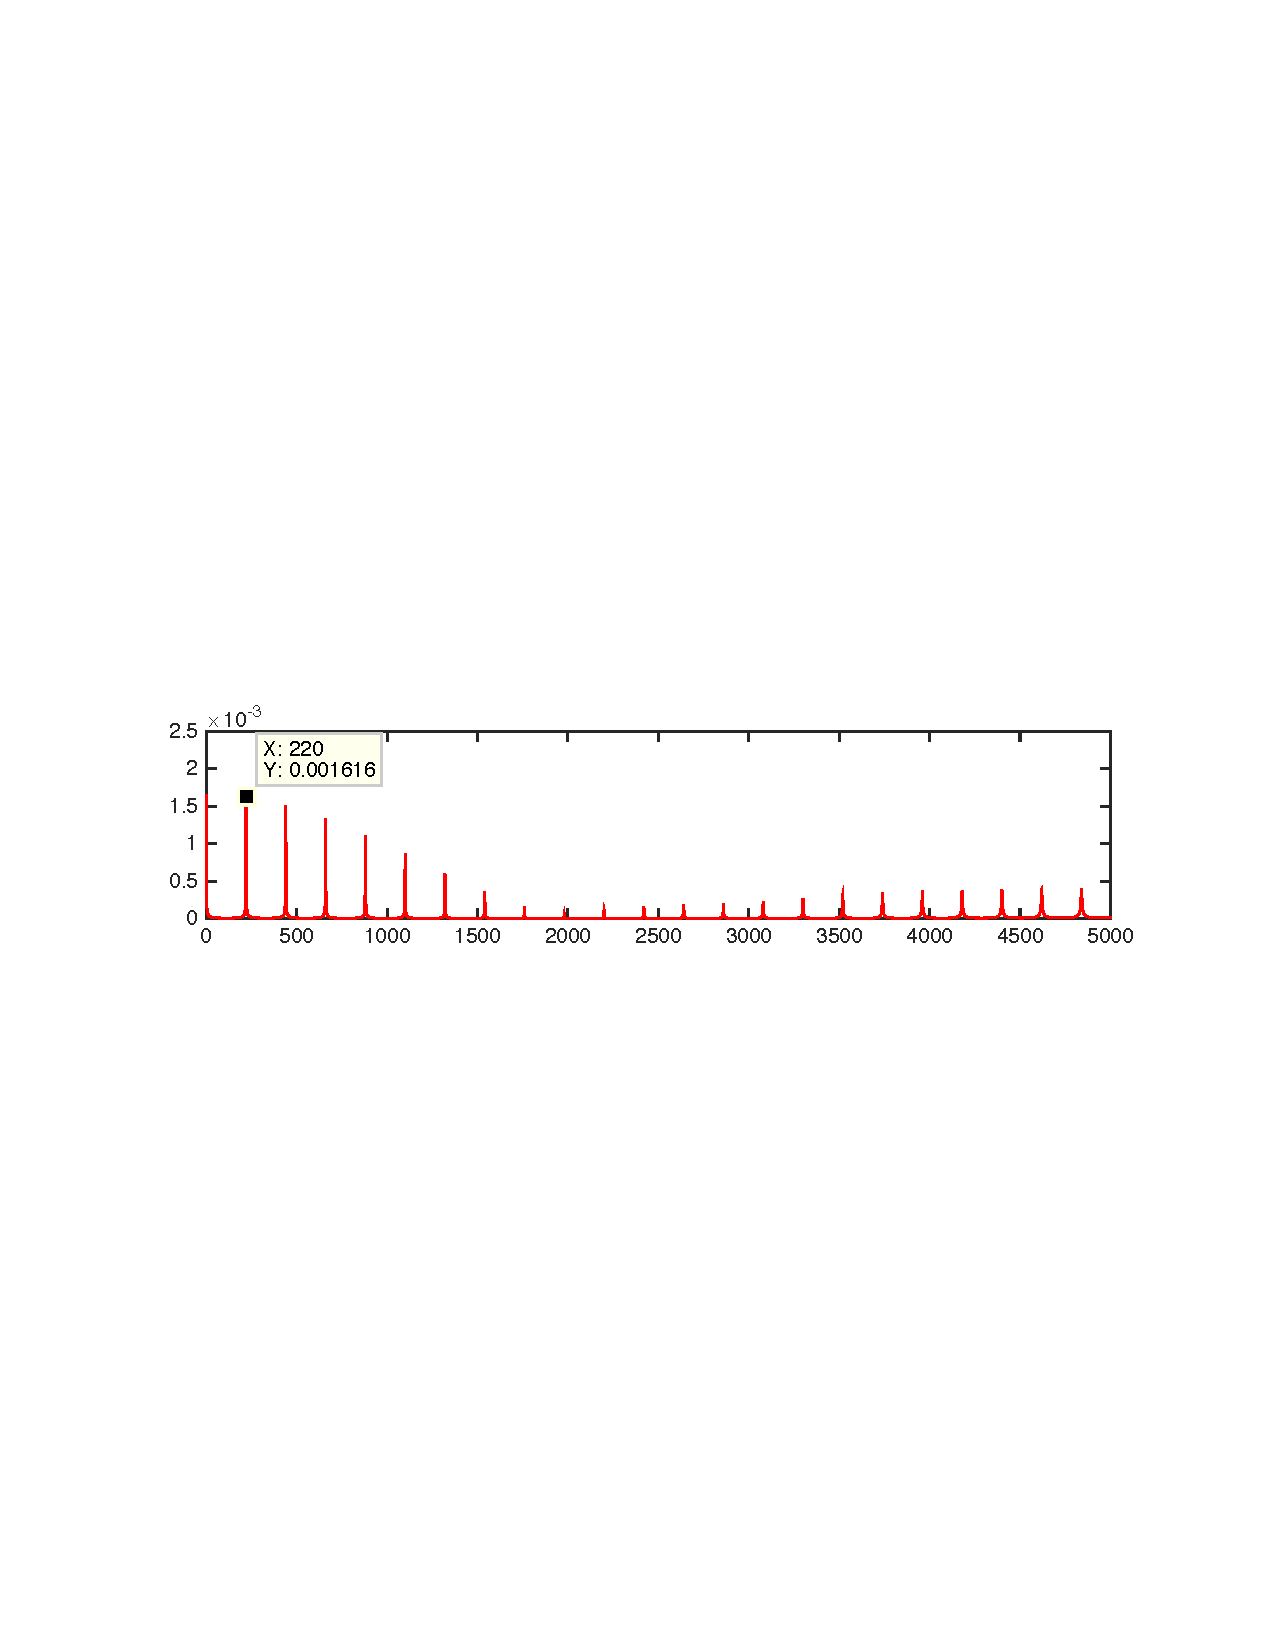
\includegraphics[scale=0.5]{onetone.pdf}
    \caption{Fourierspektrum av en grundton skapad med programmet.}
    \label{fig:onetone}
\end{figure}

\section{Slutsats}

För att visa att tonerna var rena gjordes ett fourierspektrum av grundtonen som
visas i figur~\ref{fig:onetone}. Detta gjordes på alla toner men det är inte med
i rapporten.

\section{Reflektion}

Tycker det är konstigt att denna laborationen är så tätt inpå labration 6.

\section{Bilagor, matlabkod}
\label{sec:bilagor}

\subsection{Program}

\lstinputlisting{../fadeOut.m}
\lstinputlisting{../fastPlayer.m}
\lstinputlisting{../fastTone.m}
\lstinputlisting{../filtered.m}
\lstinputlisting{../getFreq.m}
\lstinputlisting{../getKeyTones.m}
\lstinputlisting{../getSpacing.m}
\lstinputlisting{../imageToChroma.m}
\lstinputlisting{../newTone.m}
\lstinputlisting{../normalize.m}
\lstinputlisting{../raise.m}


\end{document}
